\chapter{Security View}

As one of the main concerns of the acquirer (stakeholder) is for the final system to be as secure as possible, both in
terms of information confidentiality and in terms of having increased protection from malicious users, we have
decided to offer a separate view of this architecture which concerns itself exactly with these security aspects. Also,
this view is not redundant in any way with the other views as it covers (in a very large proportion) matters that
are not discussed in any of the other views.

\section{User management}

One of the aspects of security which is of concern to the acquirers is making sure that access to parts or all of the
system can be restricted only to authenticated users. In order to cope with this requirement we propose a 2-level
user management strategy which we see as fit for this particular case. While deciding upon the particular security
model to use, we also took into account the acquirer's concern of limiting the changes to the system (and,
consequently, the costs implied thereby) to a manageable level.

The first of these two levels deals with the situation that by the end of phase 2 of development both customers
themselves  and Call-Center employees can access the functionality of the system through the Internet. However,
we have assumed that Call-Center employees (should) have access to an super set of the facilities the customers
(should) have access to. This implies that a distinction has to be made between the two kinds of users. Also,
we envision that it is possible that in the (perhaps near) future, the system will be upgraded so that even more
categories of SureThing's employees than merely Call-Center employees will be able to use it in a web-based manner.
Clearly, such categories of users will have to be distinguished as well one from another and also from the simple
customers. We have therefore decided to enforce authentication and checking of all actions performed by any users
so that we prevent unauthorized users from seeing information (or, even worse, modifying it) they would normally
not be allowed to.

In order to achieve this we propose that the structure described in figure \ref{fig:dbs} be created into the Oracle database
and, subsequently, write UCIS in such a way that user credentials are checked on login, stored as part of the session
and checked every time a request for performing an action is made. Such checks are to be done by the Front Controller
servlet (see Logical View) so that:

\begin{itemize}
\item the code is not duplicated in each class (so that it is easier to change, easier to test, easier to set up);
\item we avoid forgetting to include them in some of the classes.
\end{itemize}

\begin{figure}[ht]
\begin{center}
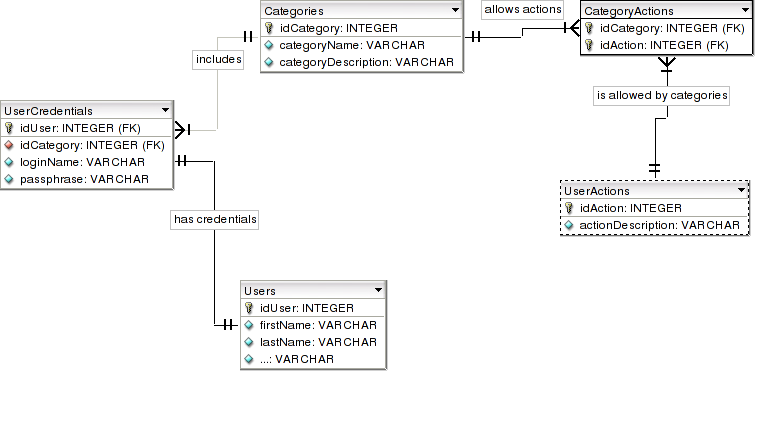
\includegraphics[width=\linewidth]{img/db-security.png}
\end{center}
\caption{Model of the security-related tables. Explanation of notations: rectangles represent tables, with the
table name and table fields being written in the rectangle. The line that appears between fields of a table
separates fields which are part of the primary key (above the line) from fields which are not part of the
primary key (below the line). Fields marked with (FK) represent foreign keys which have been exported from another table.
The names of the fields are separated from their respective types by a colon. Lines between rectangles represent
relationships between tables. Thin(ner) lines represent non-identifying relationships, while thick(er) lines
represent identifying relationships. The symbols at the end of the lines indicate multiplicity. Two parallel lines
show a multiplicity of \textit{1}, while a line and a three other converging lines show a multiplicity of \textit{n}.
Finally, relationship names should be read like: $<$table exporting foreign key$>$ $<$relationship name$>$
$<$table importing foreign key$>$.}
\label{fig:dbs}
\end{figure}

Security rights should be associated with actions in a database table (as opposed to in a configuration file) - here called
CategoryActions - so that scalability is further ensured (i.e. we don't have to worry about having all the copies of the
configuration files consistent because all the information will be in just one place, namely in the database). In order
to avoid large number of accesses to the database, the Front Controller servlet will read this information on initialization
once and use it throughout its lifetime. This means that when the security rights are modified, all the running Front
Controller servlets have to be restarted.

The second level of security is the database access security level, i.e. using the database user checks which Oracle allows.
A database user is to be created for each category of employee or customer that accesses the IT system and configure
subsystems, depending on what category of users use them, to use the particular database user which is associated
with the category of employee using the subsystem. As such, PROFI will use, for example, the accountant database user,
CHIPS will use, for example, the claim handler database user and so on. This second level of security is introduced to deal
with the acquirer's concern of wanting to achieve a certain degree of internal control of access to data (i.e., allow certain
categories of employees access only to certain parts of the database). Although not very flexible, we believe that this scheme
is appropriate as a first step in achieving internal security. Of course, employees which don't access the system through
the Internet could be included in the first level scheme as well, but this would imply a lot of changes to all of the current
subsystems (CHIPS, BuRP and PROFI), which the acquirer wants to avoid.

\section{Protection against malicious users}

This second section deals with the acquirer's concern that his customers' confidentiality is ensured, that the internal system
is well protected against attacks and that all sensitive information sent over the network is protected from eavesdropping.
In order to address these concerns we propose a number of security measures which we recommend that are taken when
developing and deploying the system.

To provide customer confidentiality as well as secure authentication for all users which access the company's web site
through the Internet, the HTTPS (i.e., HTTP using Secure Sockets Layer) protocol should be used for all such sensitive
communication. It is not vital that HTTPS be used for all communication that takes place over the public network, but it
is vital that at least authentication of users and communication of confidential customer information use HTTPS.

The company's network should be configured in such a way that none of the company's machines except the web server(s)
are accessible from the Internet. This will introduce an additional level of protection in the way of possible attackers, as
they would first have to gain access to the machines running the web server(s) and only then could they start attacking
internal machines. In order to achieve this, we recommend that the load balancer for the web server that is proposed in the
physical view be bought from the very beginning (even if currently the company does not require more than one web
server to handle the customer load). As the load balancer is actually an extended router, it can be configured to serve as
a firewall which denies access to all ports other than 80 (or whatever port the web server(s) are running on). Sure enough,
once the customer load increases and the company buys a second machine to run a web server to deal with it, the load
balancer will continue to behave as a firewall as a secondary purpose and also start acting primarily as a load balancer.
This suggestion comes as a solution for the acquirer's concern of protecting its internal network from attacks.

Since if the previous suggestion is put into practice the web server becomes the only gate of access to the internal network,
two additional measures can be taken for further securization of the company's network:

\begin{itemize}
\item use a secure operating system on the machines running the web server (e.g. OpenBSD, NetBSD);
\item use a secure web server to run the application (e.g. the Apache web server).
\end{itemize}

In addition from being secure, such software would also help reduce the costs as any of the above mentioned systems
are free.

Another aspect which we have in mind is to also secure the communication over the (current) 2 MBit lines connecting
the IT center from the other 4 locations where the company runs its business. In order to achieve this, we recommend
configuring the networks in the 5 locations as a large Virtual Private Network (VPN) and make sure that the routers
which provide the connections (at all ends) use IPSec for all data communication between the locations. This way, any
possible naive eavesdropping can be avoided, while ensuring a certain level of protection against less naive attempts
as well.

Last, but not least, we can also suggest an additional measure of protection against attackers gaining access to the most
sensitive of the company's data by installing a (software) firewall on the machine running the Oracle database and
configuring it in such a way that all attempts of accessing the database made from machines other than the ones running
the UCIS system and the STIFF system are disallowed. In this way, even if, say, an attacker gained control of some of
the internal machines (other than the ones running UCIS/STIFF), it would have a hard time accessing company data
which is stored in the Oracle database.